\section{Introduction}

Distributed Cyber-Physical Systems (CPS) are hard to develop
hardware/software for; because the software is coupled with the
hardware and the physical system, software testing and deployment may
be difficult - a problem only exacerbated by distributing the system.
All systems require rigorous testing before final deployment, but may
not be able to be tested easily in the lab or may not be testable in
the real world without first providing the assurances that testing
produces, especially with respect to reliability and fail-safety.
Examples of these systems include unmanned aerial vehicle (UAV)/
unmanned underwater vehicle (UUV) systems, fractionated satellite
clusters \cite{brown2006fractionated}, and networks of autonomous vehicles, all of which require
strict guarantees about not only the performance of the system, but
also the reliability of the system.

Developing systems in a design-test-integrate-iterate methodology is
standard practice especially for hardware systems, where electrical
and mechanical components can be prototyped and unit-tested before
performing higher-level system integration testing.  This development
approach becomes more challenging when developing software however,
since there do not exist well-adopted pervasive standard interfaces
and design principles for software.

Emerging industry standards and collaborations are progressing towards
component-based system development and reuse, \emph{e.g.}
AUTOSAR\cite{autosar} in the automotive industry.  As these systems
are becoming increasingly more reliant on collections of software and
hardware components which must interact, they enable more advanced
features, and performance, but must still meet stringent safety
requirements and as a consequence require more thorough integration
testing.  Comprehensive full systems integration is required for
system analysis and deployment, and the development of relevant
testing system architectures enables expedited iterative integration.
Developing these systems manually, by prototyping individual
components and composing them can be expensive, time consuming and
error prone, so tools and techniques are needed to expedite this
process.

Examples of such systems which can be prototyped and tested using this
architecture are (1) autonomous cars, (2) controllers for continuous
and discrete manufacturing plants, and (3) UAV swarms.  Each of these
systems is characterized as a distributed CPS in which embedded
controllers are networked to collectively control a system through
cooperation.  Each subsystem or embedded computer senses and controls
a specific aspect of the overall system and cooperates to achieve the
overall system goal.  For instance, the autonomous car's subsystems of
global navigation, pedestrian detection, lane detection, engine
control, brake control, and steering control all must communicate and
cooperate together to achieve full car autonomy.  The control
algorithms for each of these subsystems must be tested with their
sensors and actuators but also must be tested together with the rest
of the overall system.  It is these types of cooperating embedded controllers
which are a distinguishing feature of distributed CPS.

%The introduction should briefly place the study in a broad context and highlight why it is important. It should define the purpose of the work and its significance. The current state of the research field should be reviewed carefully and key publications should be cited. Please highlight controversial and diverging hypotheses when necessary. Finally, briefly mention the main aim of the work and highlight the main conclusions. As far as possible, please keep the introduction comprehensible to scientists outside your particular field of research. Citing a journal paper \cite{ref-journal}. And now citing a book reference \cite{ref-book}.

% What is ROS?
In the field of Robotics, adoption of Robot Operating System (ROS)
\cite{ROS} has become widely prominent. ROS is a meta-operating system
framework that facilitates robotic system development. ROS is widely
used in various fields of robotics including industrial robotics, UAV
swarms and low-power image processing devices. The open source
multi-platform support of ROS has made it a requirement in several
DARPA robotics projects including the \emph{DARPA Robotics Challenge}
\cite{DARPA_Robotics_Challenge}.
% What does ROS provide: ROS enables the deployment of a network of interacting processes, that communicate using the ROS middleware infrastructure. ROS nodes can contact each other using different types of interaction patterns including synchronous remote method invocation (RMI) and asynchronous message passing publish-subscribe interactions. A ROS application is a packaged set of ROS nodes that communicate through a ROS Master, where a ROS Master is a single discovery and communications broker that facilitates node-node flow setup.

% What is ROSMOD
This paper describes ROSMOD \cite{ROSMOD}, an open source development
tool suite and run-time software platform for rapid prototyping of
component-based software applications using ROS. Using ROSMOD, an
application developer can create, deploy and manage ROS applications
for distributed real-time embedded systems. We define a strict
component model, and present a model-driven development workflow with
run-time management tools to build and deploy component-based software
with ROS.
% AGSE - Tell readers about how ROSMOD is used
The utility of ROSMOD is demonstrated using a real-world case study:
an Autonomous Ground Support Equipment (AGSE) robot that was designed,
prototyped and deployed for the NASA Student Launch Competition
\cite{NASA_SL} 2014-2015. We describe the challenges and requirements,
the robotic design, the software prototyping and the overall
performance that led us to winning this competition.

% Following sections 
%The sections in this paper are organized as follows. Section \ref{sec:ROSMOD} describes the ROSMOD tool suite: The component model, modeling language, graphical user interface, code generators and deployment infrastructure. Section \ref{sec:Case_Study} describes our AGSE robot and evaluates ROSMOD. Section \ref{sec:Future_Work} describes our current efforts to improving ROSMOD support with analysis tools and run-time reconfiguration solutions. Section \ref{sec:Related_Research} presents related efforts in the field of robotics, both using ROS and other similar middleware platforms. Finally, Section \ref{sec:Conclusions} presents concluding remarks.

%%%%%%%%%%%%%%%%%%%%%%%%%%%%%%%%%%%%%%%%%%

\subsection{ROSMOD Component Model}

Software development using ROSMOD is influenced by the principles of
Model Integrated Computing\cite{sztipanovits1997model} and Component-based Software
Engineering \cite{CBSE}\cite{Heineman:01}. Large and complex systems
can be built by assembling reusable software pieces called
\emph{components}. These components are specified by well defined
execution semantics and interaction patterns.  With this model of a
component's behavior, more complex software can be created as the
composition of multiple components and a mapping between the
input/output ports of the components.  ROSMOD components contain
executable code that implement functions, manipulate state variables
and interact with other components in applications. This model is
inspired by our previous efforts with the F6COM Component Model
\cite{DREMS_CM}.

%What ROS has and what ROSMOD provides?
Here, ROSMOD is focused on improving the software development workflow
for ROS applications. ROS provides a light-weight middleware framework
for a variety of interactions between processes via a communications
broker. However, the development of ROS applications is neither
model-driven nor component-based; ROS processes, called \emph{nodes},
are assembled together into a \emph{package} and interact using the
supported set of ROS \emph{ports}. ROS defines certain types of input
and output ports that are available with either blocking or
non-blocking semantics: \emph{publish-subscribe} interactions enable
non-blocking one-to-many one-way transport of data while
\emph{client-server} interactions enable blocking send/receive
one-to-one interactions. In these interactions, the publishers and
clients act as the output ports and therefore trigger subscriber and
server input ports.  In these interactions, input ports trigger
\emph{operations} which can execute arbitrary code.  Such nodes can
also be triggered by timers for time-triggered operations
e.g. periodic camera feeds. It is important to note that ROS imposes
no design constraints or principles on the nodes; they can be any
process with any number of threads, shared memory, etc.  The goals of
ROSMOD are to provide a component model with clear execution semantics
coupled with design principles for multi-threaded distributed code,
and a model-driven development tool suite for rapid prototyping of ROS
applications, while receiving the numerous benefits of component-based
software engineering.

ROSMOD components, as shown in Figure \ref{fig:ROSMOD_Component}, can
contain a variety of ports and timers. Publisher ports publish
messages, without blocking, on a message topic. Subscriber ports
subscribe to such topics and receive all messages published on the
specified topic. This interaction implements an anonymous topic-driven
publish-subscribe message passing scheme
\cite{Eugster:2003:MFP:857076.857078}. Server ports provide an
interface to a component service. Client ports can use this interface
to request such services. Clients and servers implement a blocking
peer-to-peer synchronous remote method invocation (RMI) interaction
\cite{1008032}. Component timers can be periodic or sporadic and
allow components to trigger themselves with the specified timing
characteristics. ROSMOD components, upon deployment, are
dormant. Execution of the application is first initiated by a
timer-triggered component. The executor thread of the triggered
component wakes up and executes the \emph{trigger operation}. The
application code written in this operation may initiate other triggers
and component interactions, thus dictating the behavior of the ROSMOD
application.

\begin{figure}[h]
	\centering
        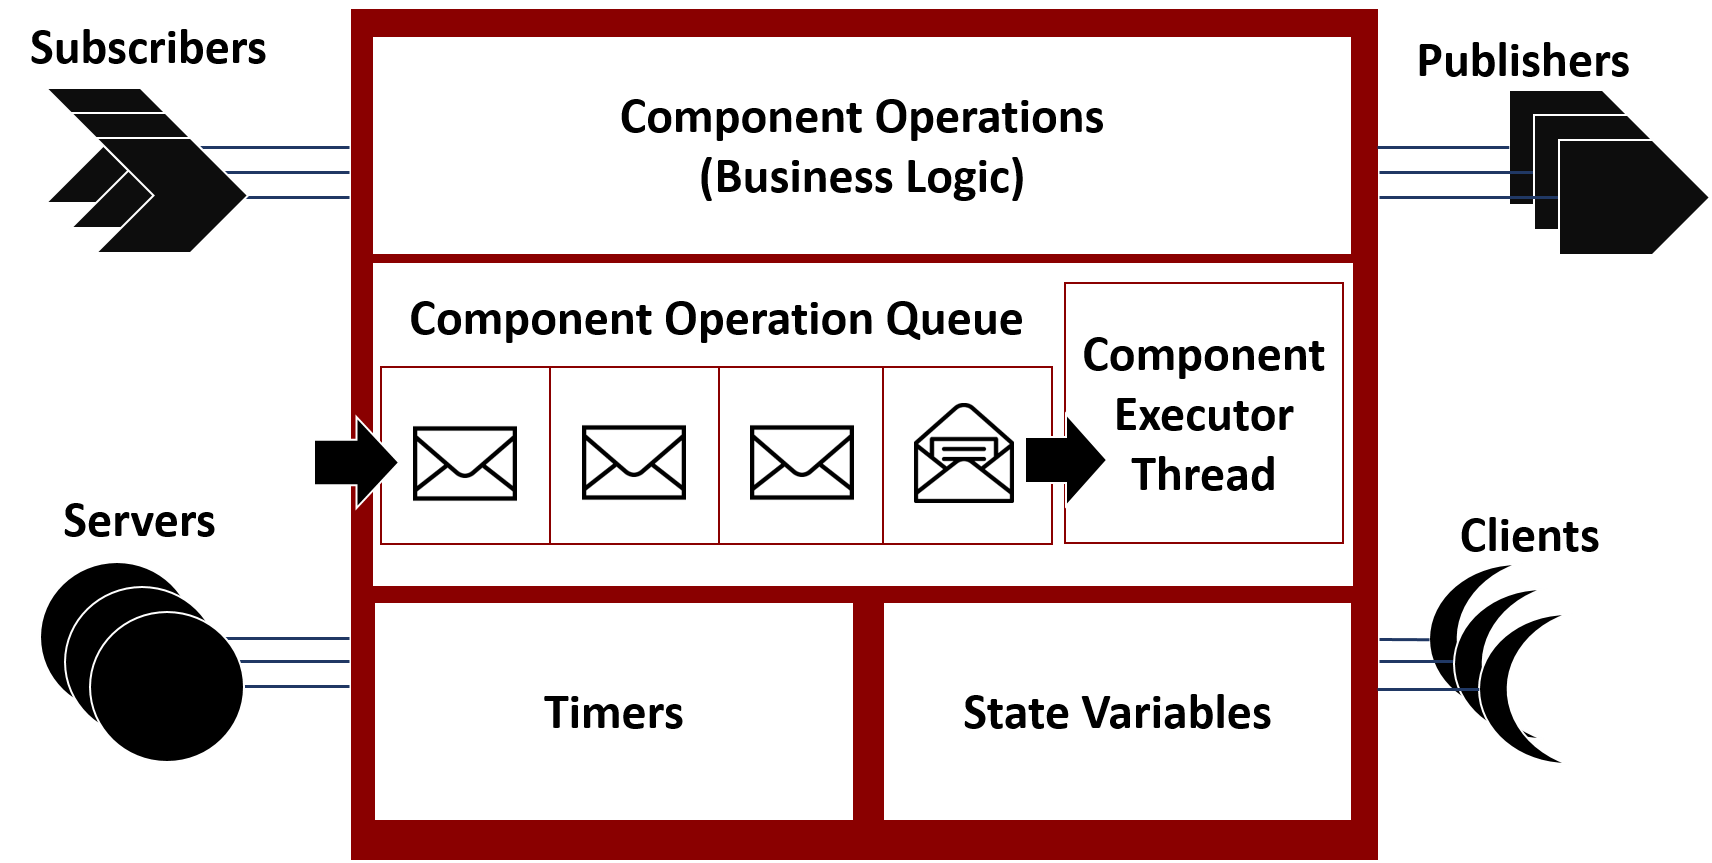
\includegraphics[width=0.8\textwidth]{Figures/ROSMOD_Component.png}
	\caption{ROSMOD Component}
	\label{fig:ROSMOD_Component}
\end{figure}

Here, an \emph{operation} is an abstraction for the different tasks
undertaken by a component. These tasks are implemented by the
component's executor code, written by the developer. Application
developers provide the functional, \emph{business-logic} code that
implements operations on the state variables. In order to service
interactions with the underlying framework and with other components,
every component is associated with a \emph{operation queue}. This
queue holds instances of operations that are ready for execution and
need to be serviced by the component. These operations service either
interaction requests (as seen on communication ports) or
library-specific requests (from the underlying framework). In each
ROSMOD component, the operation queue is processed by a single
executor thread. Multiple components may run concurrently but each
component's execution is single-threaded. Also, the component
operation queue supports several scheduling schemes including FIFO
(first-in first-out), PFIFO (priority first-in first-out) \cite{lehoczky1990fixed} and EDF
(earliest deadline first) \cite{liu1973scheduling}. Operations in the operation queue are executed using a non-preemptive scheduling scheme. This scheduling
scheme means that each operation run by the executor thread is run to
completion before the next operation in the queue is processed.  The
use of this component execution model is to enable composable,
single-threaded components which can communicate with each other
through the underlying ROS middleware without the developer having to
deal with locking shared resources or dealing with other related
multi-programming issues that typically introduce difficult to debug
errors or other run-time issues.  Again, following component-based
software design allows these components to encapsulate related
functionality into a reusable piece of software that can be shared
between projects and systems that require that functionality.

\begin{figure*}[ht]
	\centering
        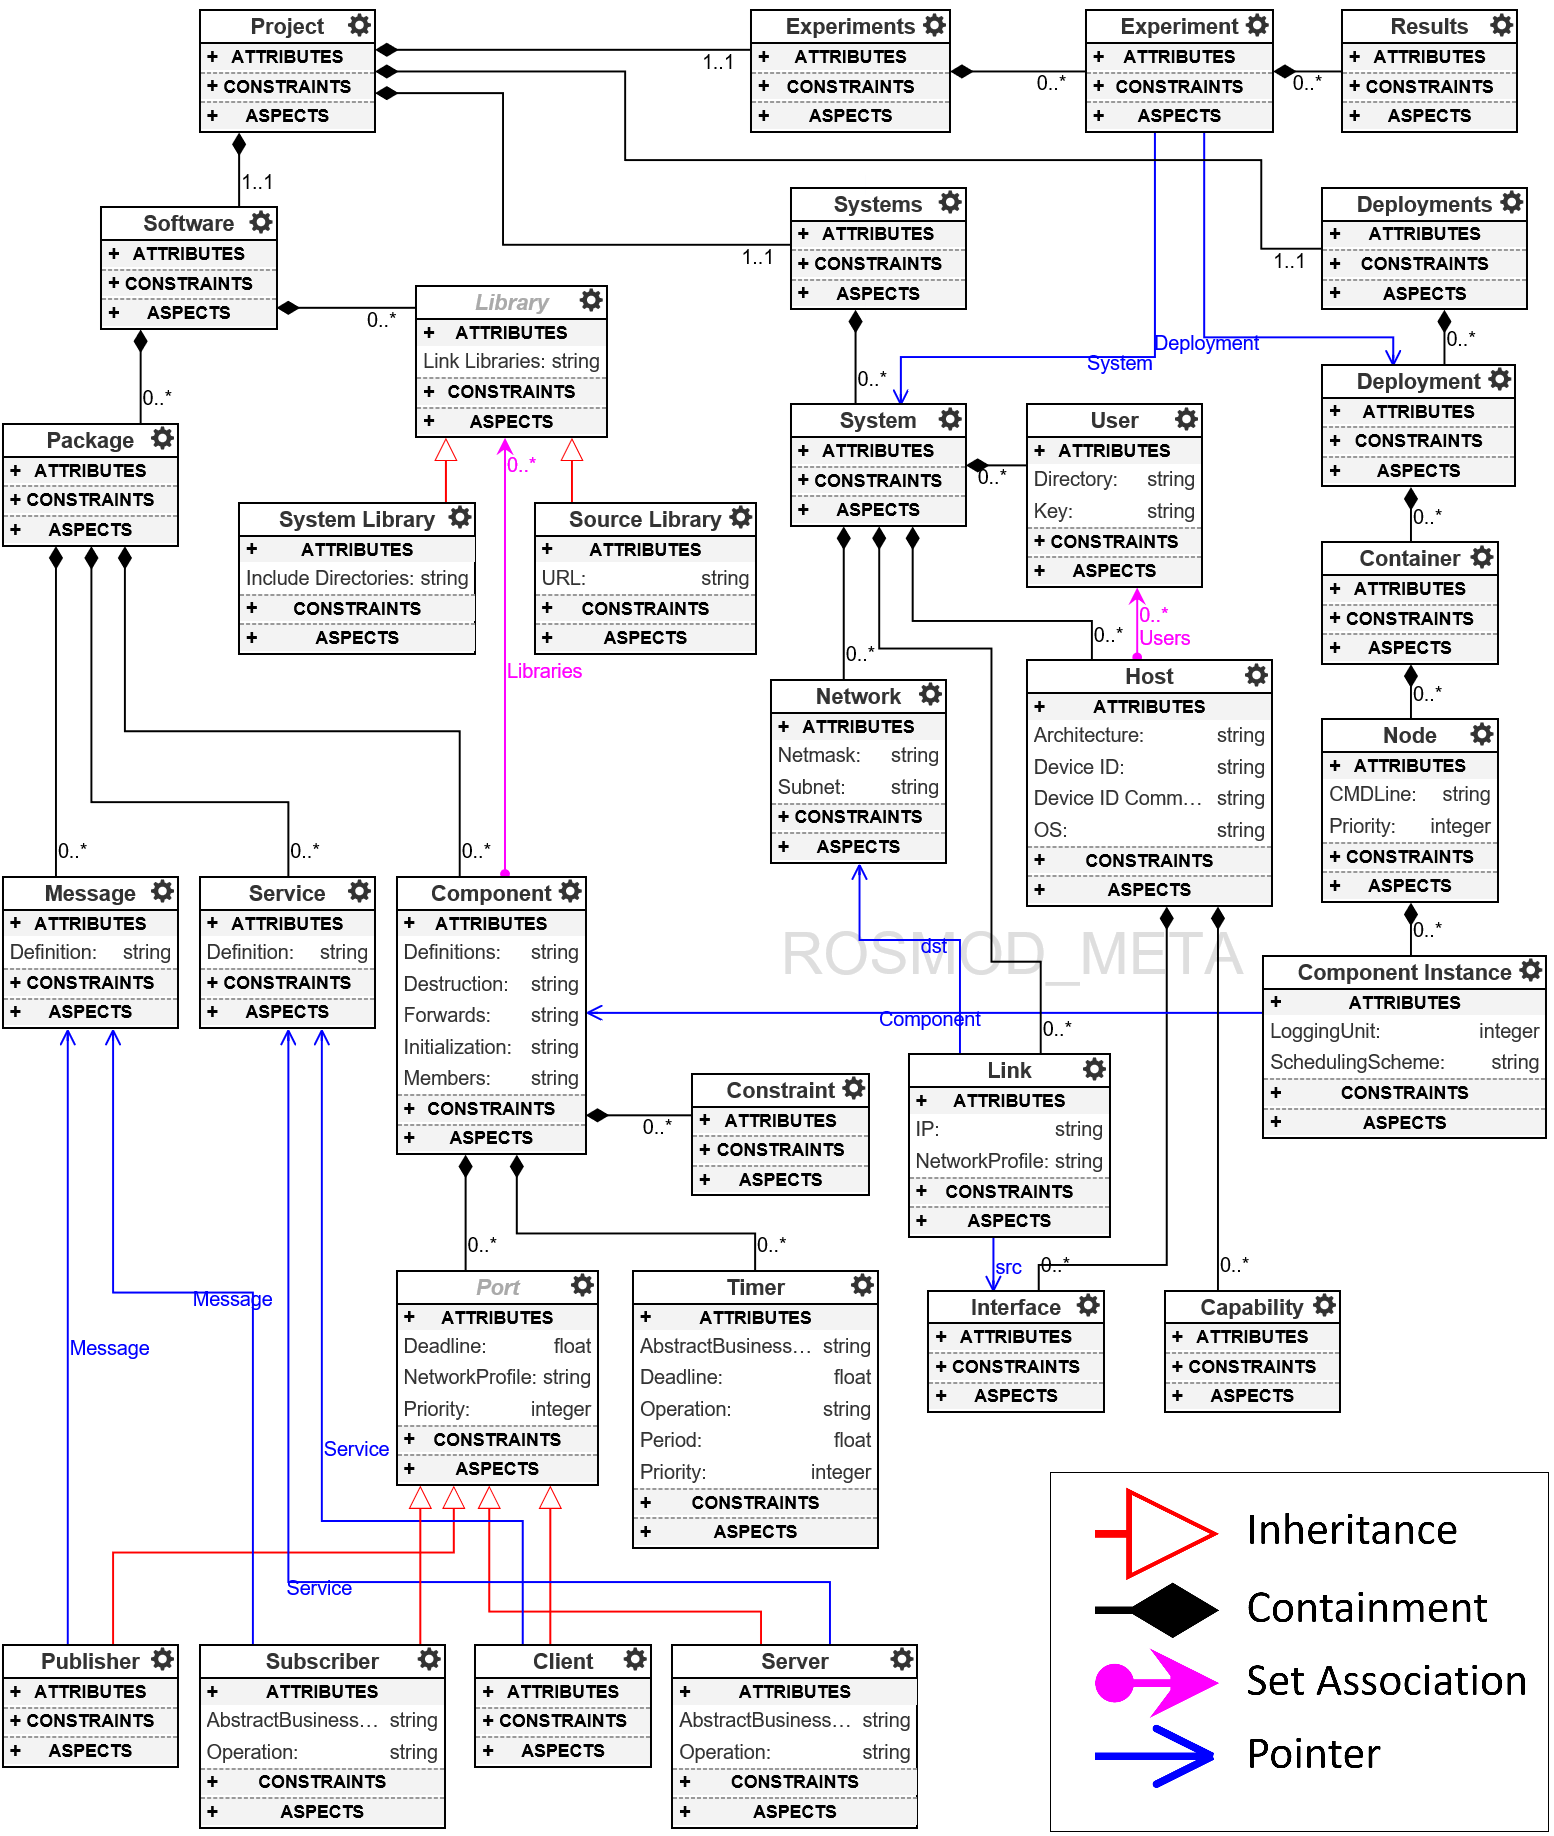
\includegraphics[width=0.82\textwidth]{./Figures/ROSMOD-Meta2.png}
	\caption{ROSMOD Metamodel.  Containment is specified from
          \emph{src} to \emph{dst} where the source has a containment
          attribute \emph{quantity}, meaning that \emph{quantity}
          objects of type \emph{src} can be contained in an object of
          type \emph{dst}. Pointers are specified as a one to one
          mapping from source to destination, using the name of the
          pointer.  Sets allow for pointer containment.  All objects
          contain a \emph{name} attribute of type \emph{string}, not
          shown for clarity.  Note: the meta-model is used to create
          the ROSMOD Modeling Language, but users do not see or
          interact with it; it is used to enforce proper model
          creation semantics. }
	\label{fig:ROSMOD_Project}	
\end{figure*}

\subsection{ROSMOD Modeling Language}

To enable the design, development, and testing of software on
distributed CPS, we have developed a modeling language specific to the
domain of distributed CPS which utilize ROS, the ROSMOD Modeling
Language (RML), shown in Figure~\ref{fig:ROSMOD_Project}.  RML
captures all the relevant aspects of the sofware, the system (hardware
and network), and the deployment which specifies how the software will
be executed on the selected system.  Using ROSMOD, developers can
create models which contain instances of the objects defined in RML.
This approach of using a domain specific modeling language to define
the semantics of the models allows us to check and enforce the models
for correctness.  Furthermore, this approach allows us to develop
generic utilities, called \emph{plugins} which can act on any models
created using ROSMOD, for instance generating and compiling the software
automatically or automatically deploying and managing the software on
the defined system.  The rest of this section goes into the specific
parts of the modeling language, called the Meta-Model, and how they
define the entities in a ROSMOD Model.

The top-level entity of RML is a \emph{Project}, which is shown in the
upper left of Figure \ref{fig:ROSMOD_Project}.  The language supports
a variety of modeling concepts that address structural and behavioral
aspects for distributed embedded platforms. ROSMOD users can create
models of software workspaces, required software libraries, embedded
devices, network topologies, component constraints and hardware
capabilities. The language also supports code development,
particularly with regards to port interface implementations i.e. the
execution code for operations owned and triggered by communication
ports or local timers. Below, we describe in detail the various
aspects of this meta-model and how these concepts are integral to
developing distributed CPS and rapid prototyping needs.

\subsubsection{Software Model}

The \emph{Software} class in Figure \ref{fig:ROSMOD_Project} models a
software workspace. A workspace, following ROS terminology, is a
collection of applications that are developed and compiled together
into binaries. Thus, each Software class can contain ROS applications,
called \emph{Packages}, and \emph{Libraries} required for the
applications. Packages consist of \emph{Messages}, \emph{Services} and
\emph{Components}. Components contain a set of pointers to Libraries
to establish dependence e.g. an \emph{ImageProcessor} component
\emph{requires} OpenCV, an open-source computer vision
library. Libraries are of two types: Source libraries and System
libraries. Source libraries are standalone archives that can be
retrieved, extracted and integrated into the software build system
with no additional changes. System libraries are assumptions made by a
software developer regarding the libraries pre-installed in the
system. Here, system refers to the embedded device on which the
component is intended to execute.

\emph{Messages} represent the ROS message description language for
describing the data values used by the ROS publish-subscribe
interactions. Similarly, \emph{Services} describe the ROS peer-to-peer
request-reply interaction pattern. Each service is characterized by a
pair of messages, \emph{request} and \emph{response}. A client entity
can call a service by sending a request message and awaiting a
response. This interaction is presented to the user as a remote
procedure call. Each ROSMOD component, as described in the component
model (Figure \ref{fig:ROSMOD_Component}), contains a finite set of
communication ports. These ports refer to messages and services to
concretize the communication interface. Components can also contain
\emph{Timers} for time-triggered operation e.g. periodically sampling
inertial measurment sensors while operating an unmanned aerial vehicle
(UAV). Lastly, components can be characterized by
\emph{Constraints}. Currently, ROSMOD constraints are a simple way to
establish hardware requirements for operation e.g. fast multi-core
processor, quadrature encoded pulse hardware, camera interface
etc. When starting such components at runtime, ROSMOD will try to map
each component to one of the available devices that satisfies all of
the component's constraints. Specifying constraints for a component
can be arbitrarily complex but currently we support simple
feature-specific constraints e.g. \emph{This component needs a device
  with atleast 12 open GPIO pins to enable motor control}. In such
cases, ROSMOD will simply scan the set of devices in the hardware
model and find a candidate host that \emph{provides} such a
\emph{capability}.  More about the deployment infrastructure and the
mapping of constraints to capabilities is described in
Section~\ref{sec:Deployment_Infrastructure}.

All requests received by a component, via subscribers or servers, and
all timed triggers can be prioritized. The prioritization is used
primarily by the component scheduler and the chosen scheduling
scheme. First-in-first-out (FIFO) scheduling of received operations
prioritizes based on the arrival time of the requests. Priority-based
FIFO resolves conflicts between received operations by using the
\emph{Priority} attribute of the relevant ports. Similary,
deadline-based schemes like the Earliest-Deadline-First (EDF) scheme
uses the \emph{deadline} of the received operation requests to resolve
conflicts and operate safely. The scheduling scheme and operation
priorities within a component are important choices to make since
these choices directly affect the efficiency and safe operation of
components. Highly critical operations need acceptable response times
for robotic systems to meet quality and timing specifications. This
design criteria is our primary motivation for integrating timing and
performance characterization techniques into our software
specification and tool suite.  The integrated performance and timing
measurement system allows for the logging and visualization of system
execution traces and to show the enqueue, dequeue, and completion of
operations being executed by the component executor thread.  As these
operations trigger each other, these traces provide valuable feedback
to the users about the performance and timing characteristics of the
system, allowing the determination of performance bottlenecks and
resource contention.

\subsubsection{System Model} 

A \emph{System Model} completely describes the hardware architecture
of a system onto which the software can be deployed. A ROSMOD Project
contains one or more \emph{Systems}. Each System contains one or
more \emph{Hosts}, one or more \emph{Users}, one or more
\emph{Networks}, and one or more \emph{Links}.  A host can contain one
or more \emph{Network Interfaces}, which connect through a link to a
network.  On this link the host's interface is assigned an IP, which
matches the subnet and netmask specification of the network.
Additionally, a host has a set of references to users, which define
the user-name, home directory, and ssh-key location for that user.
The host itself has attributes which determine what kind of processor
architecture it has, e.g. \emph{armv7l}, what operating system it is
running, and lastly a combination of Device ID and Device ID Command
which provide an additional means for specifying the type of host (and
a way to determine it), for instance specifying the difference between
a BeagleBone Black and an NVIDIA Jetson TK1 which both have armv7l
architecture but can be separated by looking at the model name in the
device tree.  Finally, a host may contain zero or more
\emph{Capabilities} to which the component constraints (described in
the previous section) are mapped.  The final relevant attribute is the
\emph{Network Profile} attribute of a link.  Using the network
profile, which is specified as a time-series of bandwdith and latency
values, we can configure the links of the network using the Linux TC
to enforce time-varying bandwidth and latency.  This network
configuration is useful when running experiments on labratory hardware
for which the network is not representative of the deployed system's
network.

\begin{figure}[h]
	\centering
        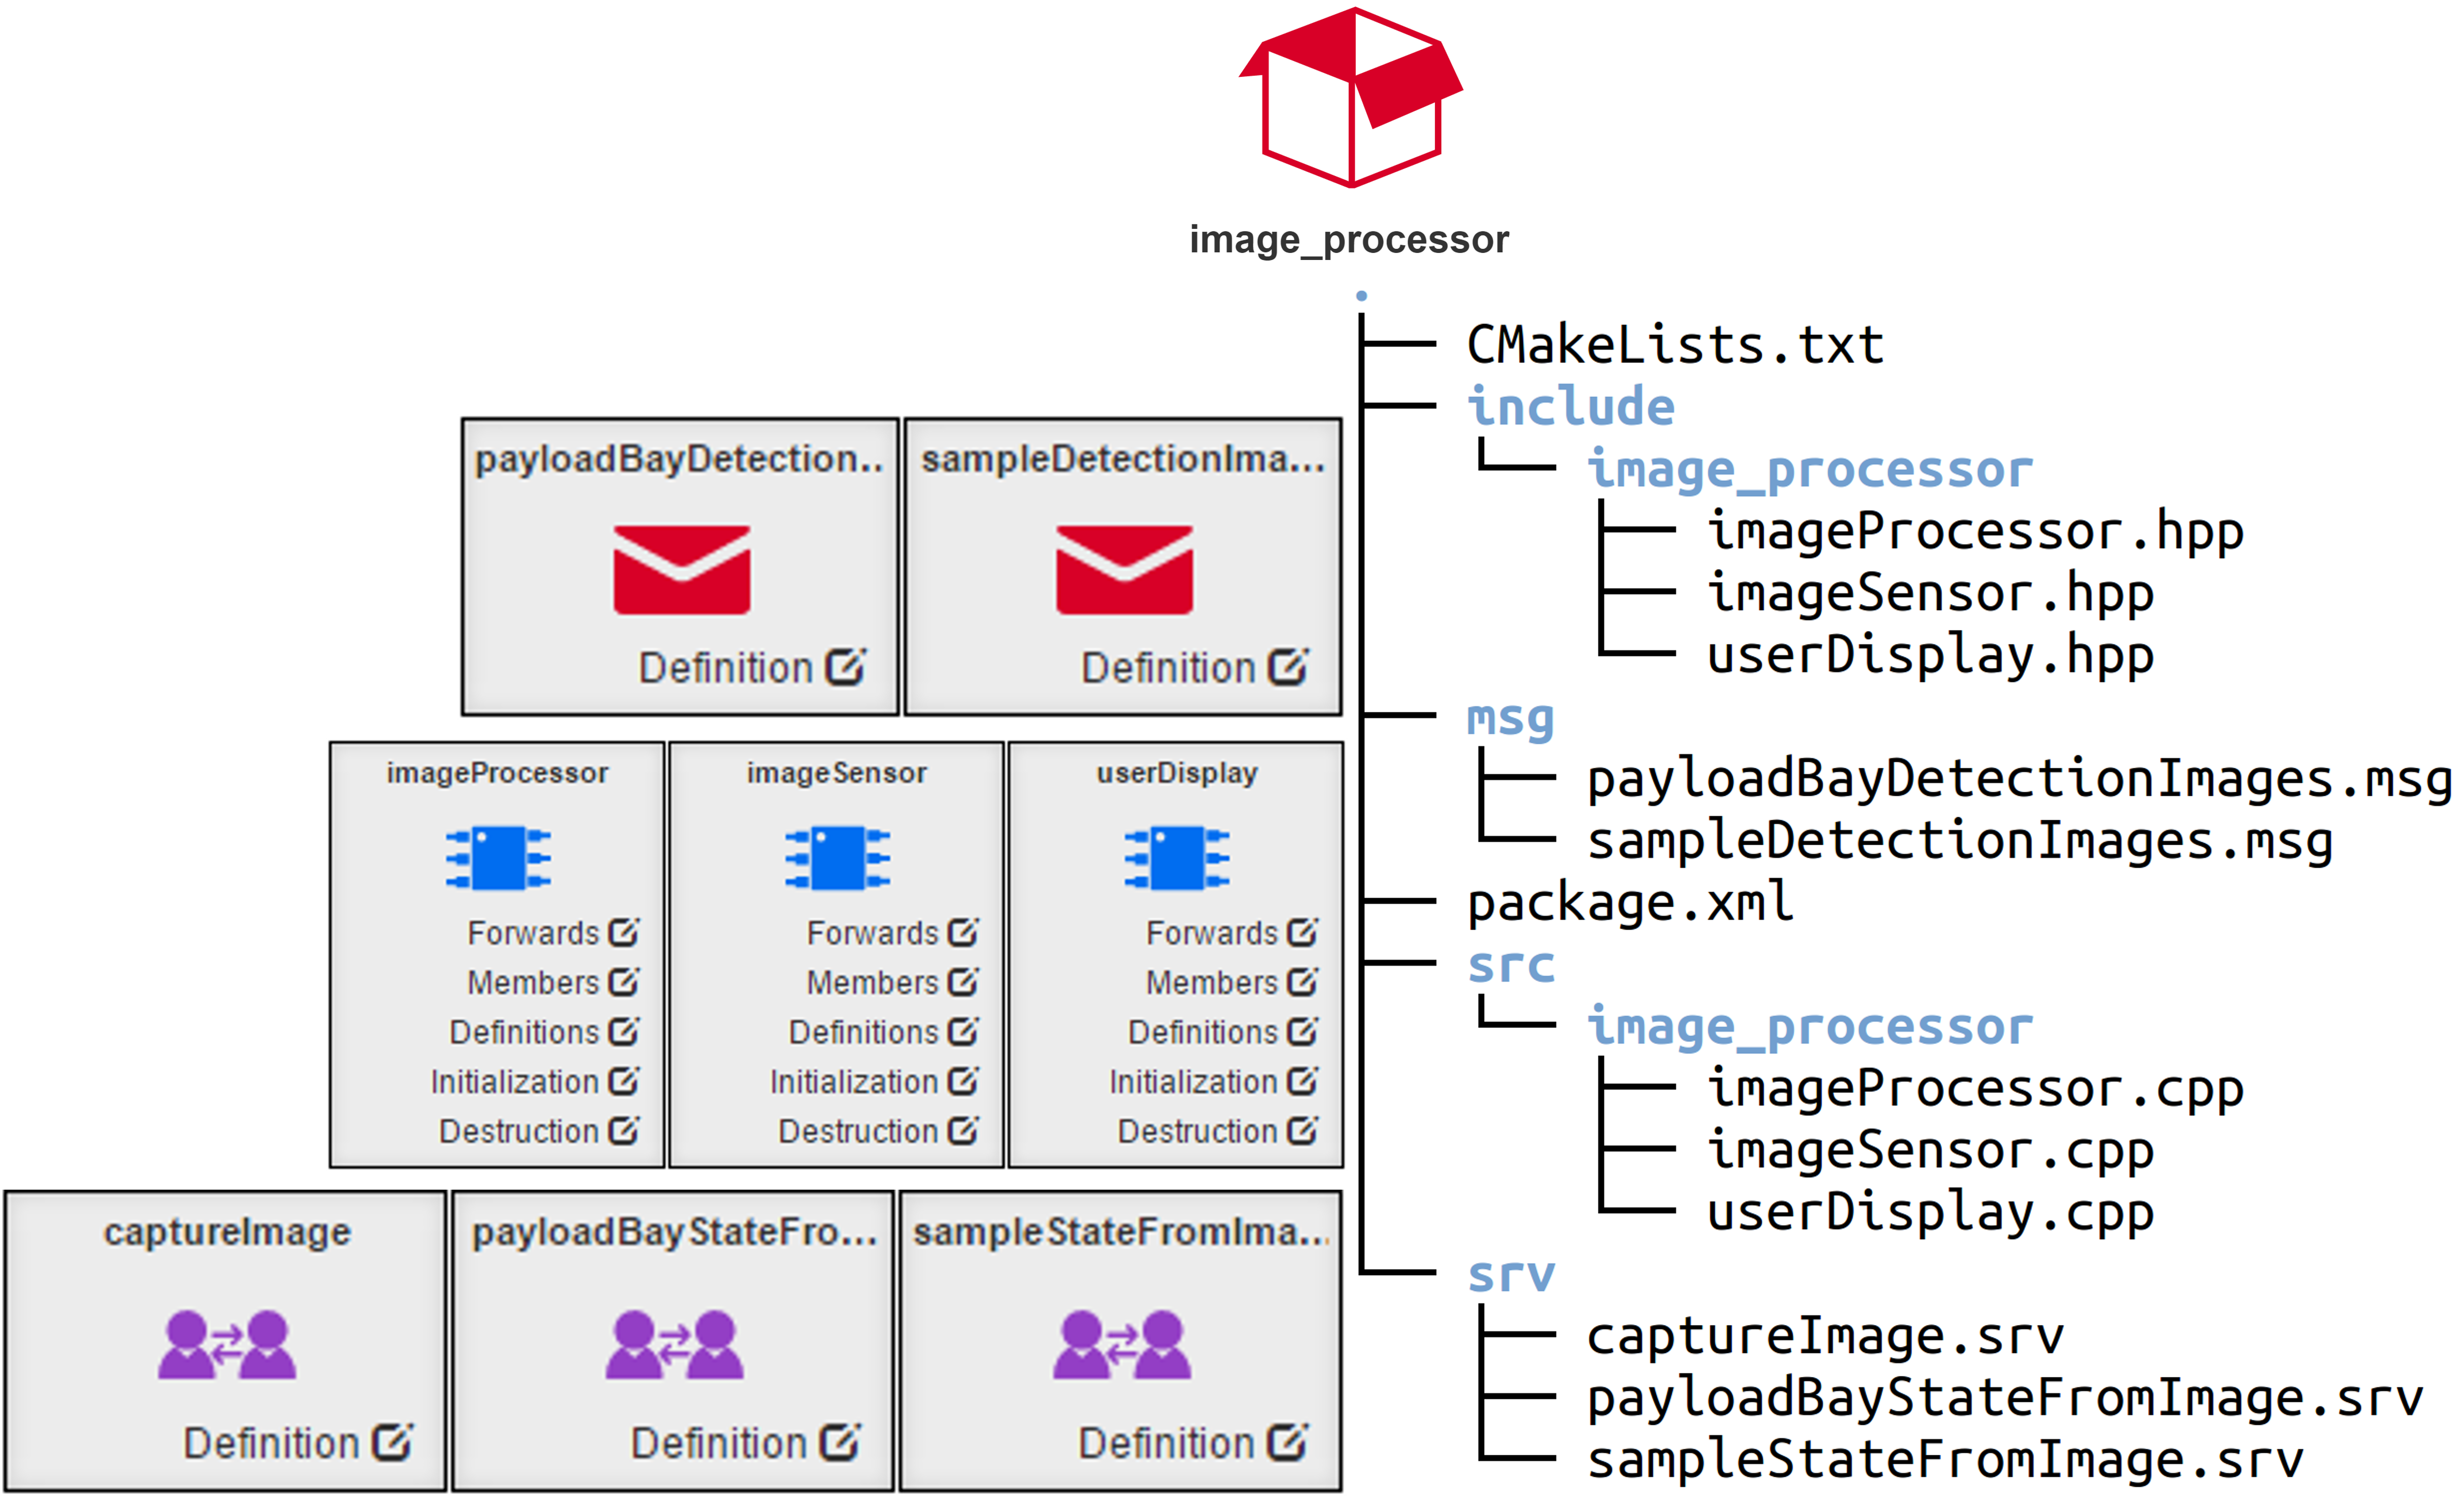
\includegraphics[width=\textwidth]{./Figures/Code_Generation.png}
	\caption{Workspace Code Generation.  In this figure, the
          \emph{image\_processor} package and its children messages
          (red), components (blue), and services (purple) are
          generated into a catkin package for compilation.  The msg
          and srv files are automatically filled out from the
          definitions of the messages and services, as are the header
          and source files for the components.}
	\label{fig:Code_Generation}
\end{figure}

\subsubsection{Deployment and Experimentation}

\emph{Deployment} refers to the act of starting application processes
on candidate hosts, where each host can provide for and satisfy all of
the constraints of the processes e.g. general purpose input/output
(GPIO) ports, CPU speed etc. Therefore, a deployment is a mapping
between application processes and system hosts on which the
application processes run.  The ROSMOD Deployment Model makes this map
a loose coupling to enable rapid testing and experimentation. Each
Deployment consists of a set of \emph{Containers}. Each container,
conceptually, is a set of processes that need to be
collocated. Containers also ensure that no process outside a container
is deployed along with the container once it has been mapped to a
host. Each container, therefore, contains a set of \emph{Nodes} (ROS
terminology for processes). In each node, application developers
instantiate one or more components previously defined in the Software
model. Following the ROSMOD component model, each such instance maps to an
executor thread that executes the operations in the component's
operation queue.  Note that the same component can be instantiated
multiple times even within the same node. Also note the container is
not mapped to a specific host within the deployment model, but rather
is automatically mapped to a host by the deployment infrastructure
within an \emph{Experiment}.

As shown in Figure \ref{fig:ROSMOD_Project}, each project supports a
set of \emph{Experiments}. Each experiment has pointers to one System
model and one Deployment model. The system model provides the set of
available devices and the deployment model provides the set of
containers, where each container contains a set of component
constraints that need satisfying (the union of all the container's
nodes' component constraints). ROSMOD uses these sets to find a
suitable mapping and then deploys the containers on the chosen host
devices, if a mapping can be found which satisfies all the constraints
of all the containers.  When the deployment infrastructure selects
hosts from the system model for mapping, it first checks to see which
of the system model's hosts are 1) reachable, 2) have valid login
credentials, 3) have the correct architecture, operating system, and
device ID, and 3) are not currently running any other compilation or
experiment processes from any other user.  In the case that there are
no available hosts in the system or the deployment's constraints
cannot be satisfied, the infrastructure informs the user.  Upon
successful deployment of the experiment, the infrastructure
automatically stores the specific mapping relevant to the deployed
experiment for later management and destruction. When such experiments
are stopped, ROSMOD retrieves the component logs from the hosts and
displays results. We are currently working on improving our runtime
monitoring features to enable real-time component execution plots and
network performance measurements at runtime.

Such a loose coupling between the deployment model and the system
model, along with the infrastructure automatically mapping the
containers to valid, unused hosts enables the execution of the same
deployment onto subsets of a large system, for instance running many
instances of the same deployment as separate experiments in parallel
on a large cluster of embedded devices.  Additionally such a loose
coupling enables redeployment onto a completely different system by
simply changing the experiment's system model reference; the
infrastructure will automatically verify that the new system meets the
constraints of the deployment and has available hosts.

\subsection{Software Infrastructure} 

The ROSMOD software infrastructure provides the user with the tools to
generate source code corresponding to the software model, compile that
source code to produce binaries that can run on the hosts defined in
the system models, and also generate documentation for the software
and associated libraries.

\subsubsection{ROSMOD Workspace}
\label{sec:code_generation}

The Software generator in ROSMOD is a plugin that produces a complete
ROSMOD workspace. The application software, as defined in the model,
is a collection of packages, each with messages, services, components
and required libraries. When invoking the workspace code generation,
ROSMOD first generates the ROSMOD packages including C++ classes for
each component, package-specific messages and services, and logging
and XML parser-specific files. Then, for each external library, the
URL of the library archive is used to fetch the library and inject
this code as a package into the generated workspace. Assuming the
library is stable and the target devices have the necessary system
libraries, this generated code compiles without errors out of the
box. The meta-model for the software is fully specified to include
attributes for user code, the business logic for the components'
operations, additional class members, etc. Because these pieces of
user code are all captured within the model, they are placed into the
proper sections of the generated code.  For this reason, it is not
necessary to alter the generated code before compilation into
binaries.  If the user chooses, the software infrastructure for ROSMOD
will automatically determine the different types of hosts in all the
current project's system models, determine which of those hosts are
available that match the model specifications and will compile the
source code into binaries for those architectures.  The compilation is
performed as a remote procedure on the host; therefore the compilation
will not select hosts which are currently running other compilation or
deployment processes.  To enable the user to multi-task, compilation
is an asynchronous non-blocking process allowing further interaction
with the model or other plugins.

\begin{figure}[h]
	\centering
        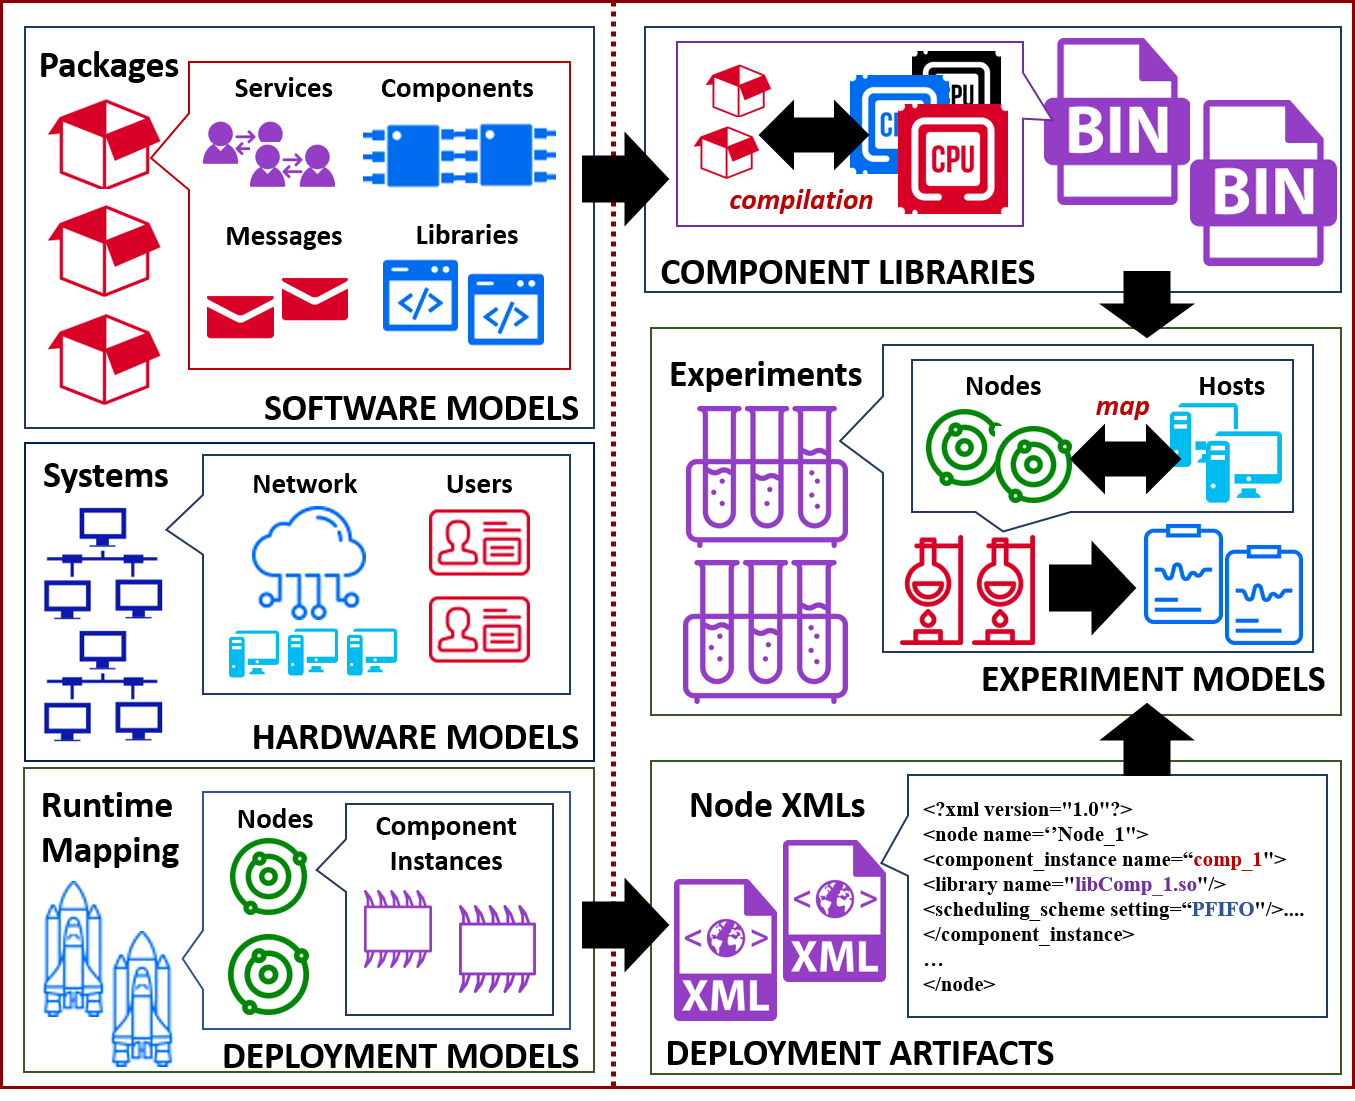
\includegraphics[width=\textwidth]{./Figures/DeploymentInfrastructure.png}
	\caption{Software Deployment Workflow}
	\label{fig:workflow}
\end{figure}

Figure \ref{fig:Code_Generation} shows the generated code tree for an
\emph{image\_processor} package. This package has three components -
\emph{userDisplay}, \emph{imageProcessor}, \emph{imageSensor}, and
associated messages and services. For each component, ROSMOD generates
a unique class that inherits from a base \emph{Component} class and
contains member objects for every component port and timer. Unlike
earlier versions of ROSMOD, this generated code is not a
skeleton. Rather, it includes all of the operation execution code
embedded in the model. So, all changes to this business logic code are
done from the model, instead of modifying a skeleton. This ensures
code consistency and avoids synchronization issues between the model
and the generated code.  Furthermore, this enables faster training and
use of the ROSMOD tool suite, since users no longer need to know into
what folders and files the generated code goes.  In the competition
version of ROSMOD, a user would have to generate the skeleton code for
the workspace, open up the relevant files manually, find the specific
places into which to place the business logic for the operations and
added members, add extra library code into the generated build files
manually, and then inform the infrastructure that the code was ready
for compilation.  This process was error prone and required detailed
knowledge of what files are generated, how to integrate libraries into
the build system, and other details that were specific to both ROS'
package system and our component implmentation.  In the current
version of ROSMOD, the user is given direct access to only the code
relevant for the specific object (component, message, service) they
are editing.  Furthermore, the library system now enables the creation
and use of libraries without knowledge of how the underlying ROSMOD
build system works.

\subsubsection{Class Documentation}

Along with the source code, ROSMOD also supports generation of
Doxygen-style documentation for all classes and files used in the
software model, including external libraries. All component files, and
library directories are scanned and the class hierarchy is constructed
from which documentation, both \emph{html} and \emph{latex}, is
automatically generated.  The generation of documentation allows for
better project maintenance, description, and training when multiple
people are working on the same project.

\subsection{Deployment Infrastructure}
\label{sec:Deployment_Infrastructure}

The workflow for software deployment is as shown Figure
\ref{fig:workflow}. After the user has generated and compiled the
software model into binary executables, they can run an experiment
that has valid deployment model and system model references. Every
ROSMOD workspace is generated with an additional \emph{node}
package. This builds a generic node executable that can dynamically
load libraries. When the software infrastructure generates and
compiles the source code for the software model, the components are
compiled into dynamically loadable libraries, one for each component
definition along with a single executable corresponding to the generic
node package. The first step the deployment infrastructure performs
when running an experiment is generating the XML files which contain
metadata about each ROS node modeled in the ROSMOD Deployment
Model. This metadata includes the component instances in each node and the
appropriate component libraries to be loaded. Based on the XML file
supplied to the node executable, the node will behave as one of the
ROS nodes in the deployment model. This allows for a reusable
framework where a generic executable (1) loads an XML file, (2)
identifies the component instances in the node, (3) finds the
necessary component libraries to load and (4) spawns the executor
threads bound to each component.

The reason for having the components be libraries that are loaded at
run-time by a node executable is 1) to help enforce separation between
each component's code, 2) to shorten the compilation time (which may
be quite long for embedded processors and complex models), and most
importantly 3) to enable the ability for users to change the mapping
of component instances to processes without the need to recompile any
of the code.  Because ROSMOD is focused on the rapid development and
deployment of reusable software components, we designed the
infrastructure to allow users to experiment with which components are
collocated within processes dynamically and rapidly iterate through
several scenarios and experiments without having to wait for code
compilations between experiments.  Finally, such a component-based
deployment framework enables unit testing and integration testing in a
very well-defined manner for the software components.  If an error
occurs during the execution of an application on a system, the user
can easily and quickly break the deployment down into sub-deployments
for unit-testing of only the relevant components to determine the
source of the error.

In the above architecture, the deployment needs three primary
ingredients: (1) the generic node executable, (2) dynamically loadable
component libraries, and (3) an XML file for each ROS node in the
deployment model. For each new node added to the deployment model, by
merely regenerating the XML files, we can establish a new
deployment. The ROS workspace is rebuilt only if new component
definitions are added to the Software Model. This architecture not
only accelerates the development process but also ensures a separation
between the Software Model (i.e. the application structure) and
deployment-specific concerns e.g. component instantiation inside ROS
nodes.

When the user has selected an experiment to run, the deployment
infrastructure first determines whether the selected deployment can
execute on the selected system.  Like the software infrastructure
described above, the deployment infrastructure queries the selected
system to validate that the system is reachable, conforms to the
model, and has available hosts for deployment (i.e. they are not
currently running any compilation or deployment processes).  Once
those available hosts have been determined, the infrastructure
attempts to map the deployment's containers to the available hosts
based on the constraints and capabilities of the two sets.  If the
constraints cannot be satisfied by the capabilities of the available
hosts, the user is informed and the deployment of the experiment is
halted.  If the capabilities of the hosts do satisfy the constraints
of the containers and their associated components, the deployment
infrastructure generates the required XML files for the deployment and
copies the XML files and the binaries over to the selected hosts,
before starting the relevant processes.  Finally, if all of those
steps are successful, the infrastructure saves the mapping into the
model for user inspection and for later teardown of the experiment.

When the user chooses to end a currently running experiment, the
deployment infrastructure verifies that the experiment is still
running before stopping the associated processes, copying the relevant
log files back, cleaning up the deployment artifacts from the hosts,
and removing the saved experiment mapping from the model.

%%%% TIMING STUFF FROM CPN : PROBABLY REMOVE
\iffalse

\subsection{Timing Analysis and Verification}
\label{sec:TAV}

\subsubsection{Problem Statement}

Consider a set of mixed-criticality component-based applications that
are distributed and deployed across a cluster of embedded computing
nodes. Each component has a set of interfaces that it exposes to other
components and to the underlying framework. Once deployed, each
component functions by executing operations observed on its component
message queue. Each component is associated with a single executor
thread that handles these operation requests. The nature of
mixed-criticality means that these executor threads are scheduled in
conjunction with a known set of highly critical system threads and
other low priority \emph{best-effort} threads. Analysis assumptions
include:

\begin{enumerate}
	\item Knowledge about the component definition, component
          assembly, communication ports, deployment mapping, temporal
          partitioning etc.
	\item Knowledge about the sequence of computation \emph{steps}
          of finite duration that are executed inside each component
          operation. This is dependent on the operation business-logic
          code written by the application developer.
	\item Knowledge of worst-case estimated time taken by the
          computational steps. There are some exceptions to this
          assumption e.g. blocking times on RMI calls cannot be
          accurately judged as these times are dependent on too many
          external factors.
\end{enumerate}

Using this knowledge about the system, the problem here is to ensure
that the temporal behavior of the composed system meets its end-to-end
timing requirements e.g. trigger-to-response times between distant
sensors and actuators. Providing this guarantee implicitly requires
that communicating components in a component assembly meet individual
timing deadlines. Following the ROSMOD component model execution, a
blocking I/O operation blocks a component from attending to any other
requests till the operation is completed. Such blocking interaction
patterns can propagate large delays to other components, especially in
a highly connected system. A useful analysis result here would not
only be in identifying end-to-end timing violations but also tracing
delays within individual components. Tracking timing violations
enables the analysis in identifying the causes for the anomalies
e.g. nontrivial circular dependencies or scheduling delays.

\subsection{Colored Petri Net-based Analysis Model}

Figure \ref{fig:hlcpn} shows a Colored Petri net (CPN) \cite{CPN}, as
modeled in CPN Tools \cite{CPNTools}, that models the structural and
behavioral semantics of ROSMOD applications. Colored Petri nets
consists of two primary modeling elements: places (circles) and
transitions (rectangles). Arcs are drawn either from places to
transitions or from transitions to places. A transition \emph{fires}
when all its input places have tokens that satisfy its conditions. By
firing, the transition removes the bound tokens from input places and
assigns tokens to all its output places, following arc-binding rules.

One of the primary reasons for choosing Colored Petri Nets over other
high-level Petri Nets such as Timed Petri Nets or other modeling
paradigms like Timed Automata is because of the powerful modeling
concepts made available by token colors. Each \emph{colored token} can
be a heterogeneous data structure such as a \emph{record} that can
contain an arbitrary number of fields. This enables modeling within a
single \emph{color-set} (C-style \texttt{struct}) system properties
such as component interaction patterns, queuing principles and even
distributed deployment. The token colors can be inspected, modified,
and manipulated by the occurring transitions and the arc
bindings. Component properties such as thread priority, port
connections and real-time requirements can be easily encoded into a
single colored token, making the model considerably concise.

\emph{Places} in this model, shown as ovals, in this model contain
colored (typed) tokens that represent the state of interest for
analysis e.g. \emph{Clocks} place holds tokens of type \emph{clocks}
maintaining information regarding the state of the clock values and
temporal partition schedule on all computing
nodes. \emph{Transitions}, shown as rectangular boxes, are responsible
for executing this model, progressing the state of the modeled system
and transferring tokens between places. \emph{Arcs}, between
transitions and places dictate the token flow and data structure
manipulations. All arcs contain emph{inscriptions}, which are
essentially function calls, written in Standard ML, that manipulate
token structures e.g. arc inscriptions in the arc from the transition
\emph{Timer\_Expiry} to the place \emph{Timers}, manipulate all timer
tokens by updating the timer expiry offsets.

\begin{figure}[h]
	\centering
        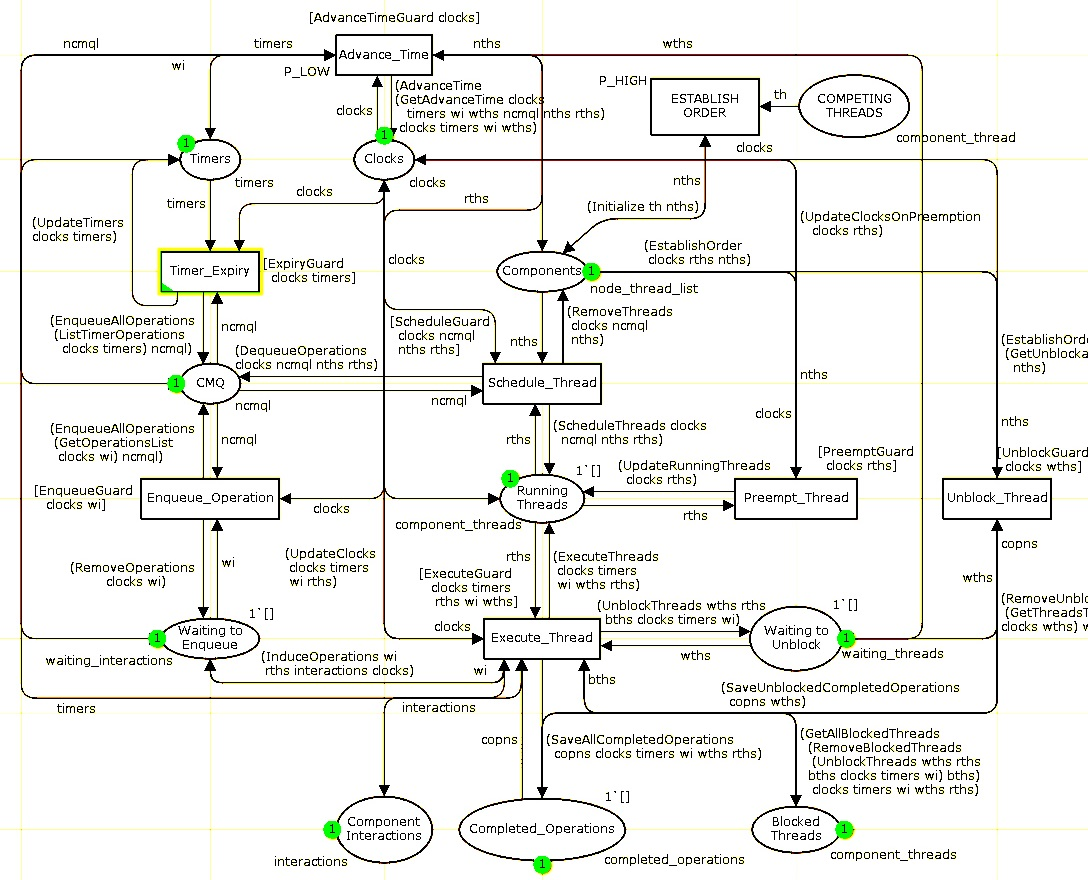
\includegraphics[width=\textwidth]{./Figures/hlcpn_cropped}
	\caption{Colored Petri Net Analysis Model}
	\label{fig:hlcpn}
\end{figure}

From the design model of the system, we generate the initial CPN
tokens that are injected into places in this analysis model. Using the
in-built state space analysis engine, we analyze the state space of
the parameterized model to compute useful system properties
e.g. processor utilization, execution time plots, deadline violations
etc. The modeling concepts in Figure \ref{fig:hlcpn} can be divided
and categorized based on system-level concepts being analyzed. Figure
\ref{fig:hlcpn_structure} shows the organizational structure of this
CPN.

\begin{figure}[h]
	\centering
        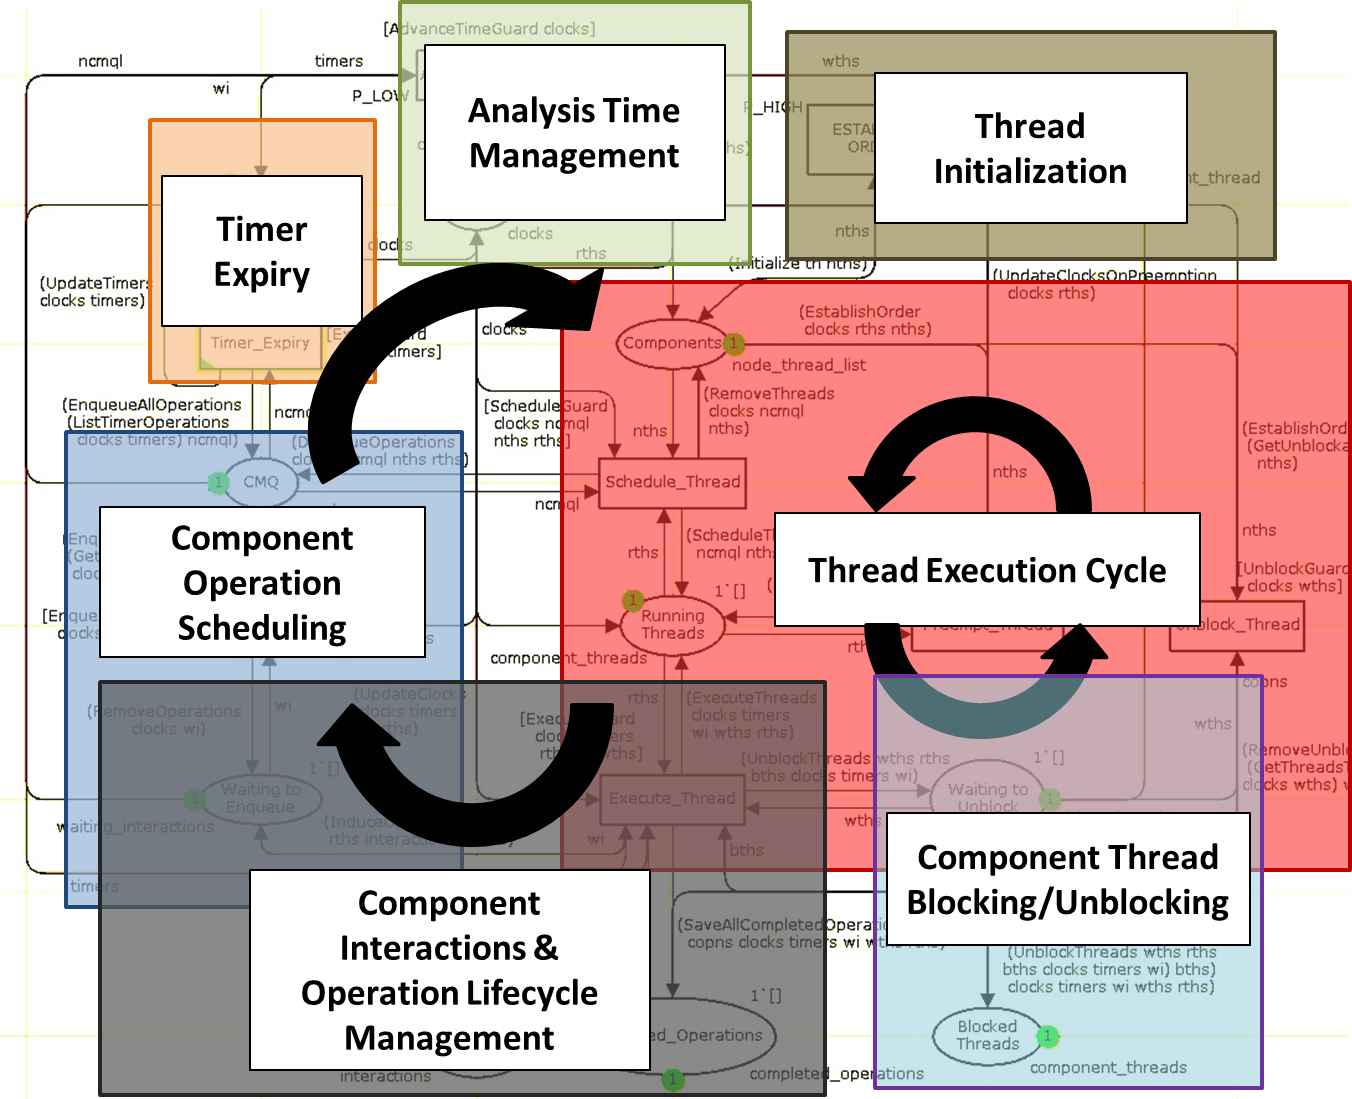
\includegraphics[width=\textwidth]{./Figures/hlcpn_structure}
	\caption{Analysis Model - Structural Aspects}
	\label{fig:hlcpn_structure}
\end{figure}

\fi
